%% It is just an empty TeX file.
%% Write your code here.
\graphicspath{{sec01/images/}{sec01/code/}}
\lstset{inputpath=sec01/code/}

\begin{frame}{Why?}

\Huge\centering Why we are studying it?
     
\end{frame}

\begin{frame}{What with command creation?}\relax
    
    For most documents you need no command creation knowledge: just using the existing.\\[3ex]
    But commands creation skill will allow you:
    \begin{itemize}
        \item Dramatically shorten the time and increase the pleasure of the process
        \item Kill the routine
        \item Create useful thing to share with others
        \item Understand and be able to change the code from templates 
        \item Usually to create a simpler UI you need a more difficult backend
         
    \end{itemize}
     
\end{frame}

\begin{frame}{To create a clear syntax for yourselves}\relax

\inputminted[firstline=90, lastline=96]{latex}{sec01/code/exExtLvl2full.tex}

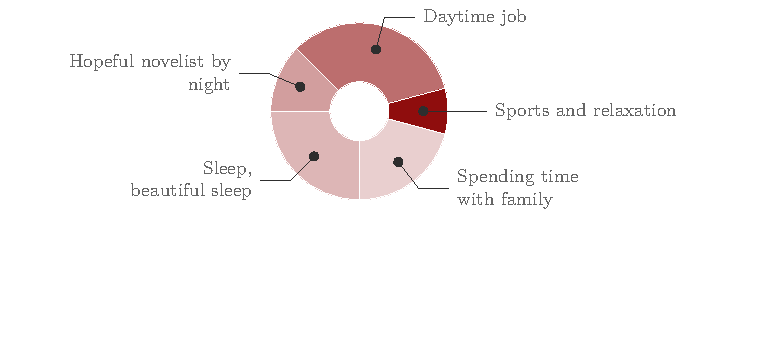
\includegraphics{exExtLvl2full}
\skfootnote{(From altaCV template)}
     
\end{frame}